\documentclass[11pt]{article}

% ------------------------------------------------------------------ packages
\usepackage[a4paper,margin=2.4cm]{geometry}
\usepackage{amsmath,amssymb}
\usepackage{graphicx}
\usepackage{booktabs}
\usepackage{array}
\usepackage{xcolor}
\usepackage{caption}
\usepackage{enumitem}
\usepackage{tikz}
\usetikzlibrary{arrows.meta,positioning,fit,backgrounds,calc,shapes.geometric}
\usepackage[colorlinks=true,linkcolor=blue!55!black,citecolor=blue!55!black,
            urlcolor=blue!55!black]{hyperref}

\definecolor{cgreen}{HTML}{2A9D4A}
\definecolor{cred}{HTML}{C0392B}
\definecolor{cblue}{HTML}{2C6FBB}
\definecolor{cgrey}{HTML}{555555}
\definecolor{boxbg}{HTML}{EEF3FA}
\definecolor{boxbg2}{HTML}{F3EEF8}

\newcommand{\code}[1]{\texttt{\small #1}}
\newcommand{\cross}{\code{cross\_asym}}
\newcommand{\dscore}{\code{directional\_score}}
\newcommand{\ifnb}{\textnormal{IFN-}\ensuremath{\beta}}
\newcommand{\nfkb}{\textnormal{NF-}\ensuremath{\kappa}\textnormal{B}}
\newcommand{\Sx}{\ensuremath{S_X}}

\captionsetup{font=small,labelfont=bf,width=0.95\linewidth}
\setlength{\parskip}{0.35em}
\setlength{\parindent}{0pt}

% ------------------------------------------------------------------ tikz styles
\tikzset{
  box/.style   = {rounded corners=2pt, draw=black!55, fill=boxbg, align=center,
                  inner sep=4pt, font=\small},
  pbox/.style  = {rounded corners=2pt, draw=black!55, fill=boxbg2, align=center,
                  inner sep=4pt, font=\small},
  data/.style  = {draw=black!45, fill=black!4, align=center, inner sep=4pt, font=\small},
  ar/.style    = {-{Stealth[length=2.4mm]}, line width=0.7pt},
  lbl/.style   = {font=\scriptsize\itshape, text=black!60},
}

% ================================================================== title
\title{\vspace{-1.2cm}\bfseries Inferring Cytokine Signaling Cascade
\emph{Direction} from a Single-Time-Point Single-Cell Snapshot\\[2pt]
\large A multiple-instance-learning pipeline and the \cross{} fix}
\author{Yam Arieli \quad\textnormal{\small(group meeting briefing / self-orientation / PI report)}}
\date{2026-05-31}

\begin{document}
\maketitle
\vspace{-0.7cm}

\begin{abstract}\noindent
\textbf{Question.} Cytokines are signaling proteins immune cells use to talk to
one another. A \emph{cascade} $X\!\to\!Y$ means stimulus $X$ causes cells to
produce $Y$. Cascade \emph{direction} is a temporal, causal property --- yet
single-cell experiments usually give us only \emph{one} snapshot in time. Can we
recover direction from a single frame? \textbf{Method.} We build a three-step
pipeline on pseudo-bulk ``pseudo-tubes'' of single cells: (A) an attention-based
multiple-instance-learning (AB-MIL) model finds \emph{coupled} cytokine pairs; (B)
per-cytokine binary classifiers + Integrated Gradients discover each cytokine's
gene signature \Sx{}; (C) a directional-asymmetry test assigns direction.
\textbf{Result.} The textbook §24 score we started from turns out to be
\emph{algebraically symmetric} and therefore direction-blind. Replacing it with
the \emph{antisymmetric} cross-engagement \cross{} $= s(a,S_b)-s(b,S_a)$ recovers
direction at \textbf{88\%} on human PBMC (24h, 17 audited cascades; vs.\ 47\% =
chance for the old score) and \textbf{86\%} on mouse BMDM at 5h
(single-frame, crystal-clear TLR-biology labels). The fix is exactly the intuition
``the upstream tube carries \emph{both} signatures; the downstream tube carries
only its own''.
\end{abstract}

% ================================================================== §1 map
\section{Project map (one page to orient)}\label{sec:map}

This project asks two linked questions about cytokine biology, and they have
become two ``paths'' (Fig.~\ref{fig:f1}). \textbf{Path A --- axis discovery}
(largely complete) asks \emph{which cytokines are coupled}: it recovered 121
cytokine coupling ``axes'' on a 91-cytokine human dataset, about half supported
by literature versus $\sim$1\% by chance. \textbf{Path B --- cascade direction}
(this report) asks the harder question: \emph{given a coupled pair, who is
upstream?} Path B stalled for months because every attempt scored at chance.
\emph{This session found why and fixed it}: the scoring statistic was symmetric
and could not encode direction; the antisymmetric \cross{} does. That single
change is the spine of this talk.

\begin{figure}[h]\centering
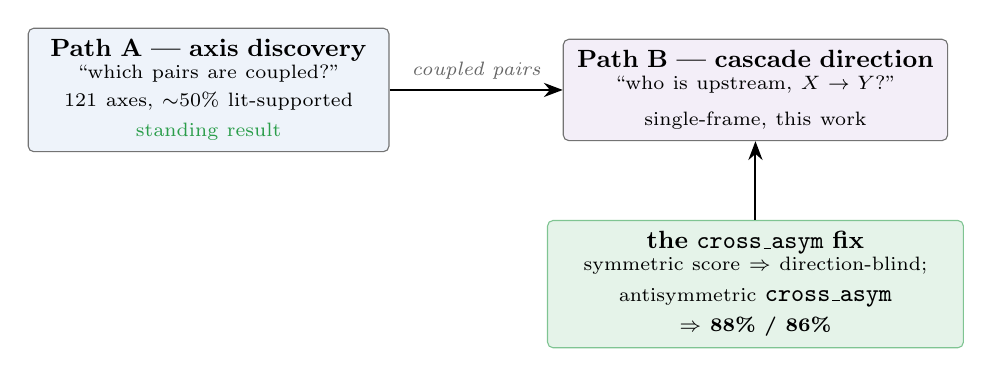
\begin{tikzpicture}[node distance=6mm]
  \node[box, text width=4.3cm] (A) {\textbf{Path A — axis discovery}\\
    \scriptsize ``which pairs are coupled?''\\[2pt]
    \scriptsize 121 axes, $\sim$50\% lit-supported\\ \scriptsize \textcolor{cgreen}{standing result}};
  \node[pbox, right=22mm of A, text width=4.6cm] (B) {\textbf{Path B — cascade direction}\\
    \scriptsize ``who is upstream, $X\!\to\!Y$?''\\[2pt]
    \scriptsize single-frame, this work};
  \node[box, below=10mm of B, text width=5.0cm, fill=cgreen!12, draw=cgreen!60] (X)
    {\textbf{the \cross{} fix}\\ \scriptsize symmetric score $\Rightarrow$ direction-blind;\\
     \scriptsize antisymmetric \cross{} $\Rightarrow$ \textbf{88\% / 86\%}};
  \draw[ar] (A) -- node[lbl,above]{coupled pairs} (B);
  \draw[ar] (X) -- (B);
\end{tikzpicture}
\caption{The two paths. Path A (coupling) feeds Path B (direction). This report
is Path B; the green node is the contribution.}\label{fig:f1}
\end{figure}

\textbf{What this report covers:} the biology and why direction-from-a-snapshot is
hard but valuable (§\ref{sec:motiv}); the data and the model (§\ref{sec:data},
§\ref{sec:method}); the result and an honest accounting of its limits
(§\ref{sec:results}--§\ref{sec:limits}); and a suggested 45-minute talk structure
(§\ref{sec:talk}). Exact hyperparameters and equations are in the appendices.

% ================================================================== §2 motivation
\section{Motivation: the biological question}\label{sec:motiv}

\subsection{A five-minute biology primer}
Every cell carries the same DNA but \emph{expresses} a different subset of genes;
the set of currently-active genes (the \emph{transcriptome}) is the cell's state.
\textbf{Cytokines} are small secreted proteins --- IFN-$\beta$, TNF, the
interleukins (IL-x) --- that immune cells use to coordinate a response. When a
cytokine $X$ binds its receptor on a target cell, it triggers an intracellular
\emph{signaling pathway} (a relay of proteins) that switches on a characteristic
set of genes, $X$'s \emph{signature} \Sx{}.

A \textbf{cascade} is when one cytokine begets another (Fig.~\ref{fig:f2}):
$X$ stimulates a cell, the cell's program includes \emph{producing and secreting}
cytokine $Y$, and $Y$ then drives \emph{its} program in neighbours. Cascades are
the wiring diagram of the immune system. Knowing the \emph{direction} of an edge
($X\!\to\!Y$ vs.\ $Y\!\to\!X$) is knowing causality --- which is what you need to
choose a drug target.

\begin{figure}[h]\centering
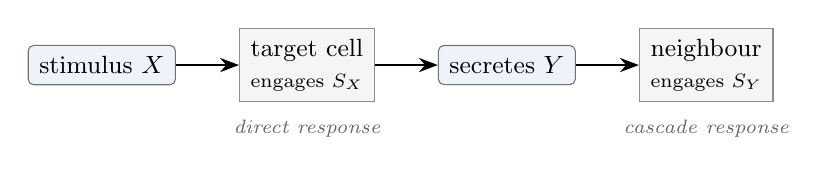
\begin{tikzpicture}[node distance=8mm]
  \node[box] (st) {stimulus $X$};
  \node[data, right=of st] (c1) {target cell\\ \scriptsize engages $S_X$};
  \node[box, right=of c1] (y) {secretes $Y$};
  \node[data, right=of y] (c2) {neighbour\\ \scriptsize engages $S_Y$};
  \draw[ar] (st)--(c1); \draw[ar] (c1)--(y); \draw[ar] (y)--(c2);
  \node[lbl, below=1mm of c1] {direct response};
  \node[lbl, below=1mm of c2] {cascade response};
\end{tikzpicture}
\caption{A cascade $X\!\to\!Y$: $X$'s target cells run $S_X$ \emph{and} make $Y$;
$Y$ then runs $S_Y$ in other cells. The asymmetry we exploit: the $X$-tube ends up
carrying both $S_X$ and $S_Y$, the $Y$-tube only $S_Y$.}\label{fig:f2}
\end{figure}

\subsection{The question and why it is hard}
We measure cells with single-cell RNA sequencing, which gives a \emph{snapshot}:
the transcriptome of thousands of cells at \emph{one} moment after stimulation
(Fig.~\ref{fig:f3}). Direction is a property of \emph{time} --- $X$ rises before
$Y$ --- so the naive view is that a single frame cannot reveal it. A full
time-course (sample every hour for many hours, every condition, replicated) would
make direction trivial, but it is expensive, and many valuable datasets are
single-frame. \textbf{The bet of this project: a single frame already contains a
\emph{spatial-in-gene-space} fingerprint of direction}, because the upstream
stimulus's cells carry the downstream signature too, while the converse does not.

\begin{figure}[h]\centering
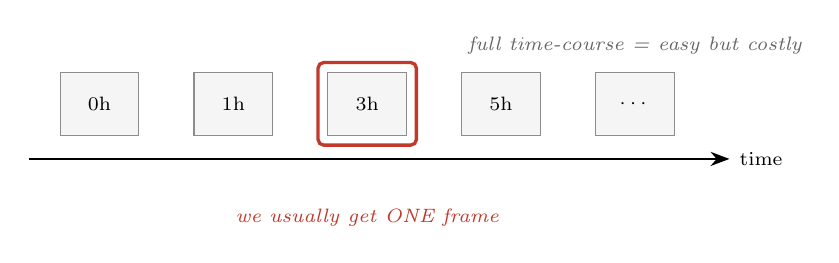
\begin{tikzpicture}[node distance=5mm]
  \foreach \i/\t in {0/0h,1/1h,2/3h,3/5h,4/$\cdots$} {
     \node[data, minimum width=1.0cm, minimum height=0.8cm] (f\i) at (\i*1.7,0) {\scriptsize \t};
  }
  \draw[ar] (-0.9,-0.7) -- (8.0,-0.7) node[right]{\scriptsize time};
  \node[draw=cred, very thick, rounded corners=2pt, fit=(f2)] (hl) {};
  \node[lbl, below=8mm of f2, text=cred] {we usually get ONE frame};
  \node[lbl, above=1mm of f4] {full time-course = easy but costly};
\end{tikzpicture}
\caption{The challenge. A time-course makes direction trivial; a single snapshot
(red) discards the time axis. We ask whether direction survives in one frame.}
\label{fig:f3}
\end{figure}

\textbf{Why it matters.} (i) Direction $=$ causality $=$ candidate intervention
points. (ii) It unlocks the many single-time-point datasets already deposited.
(iii) The method is generic: any system with labeled stimuli that participate in
cascades (not just cytokines) could be analysed the same way.

% ================================================================== §3 data
\section{Data: cells, pseudo-tubes, and two datasets}\label{sec:data}

\subsection{From cells to ``pseudo-tubes''}
Single-cell RNA-seq yields a (cells $\times$ genes) matrix per condition. A single
cell is noisy, and our label (``which stimulus was applied'') is defined at the
\emph{sample} level, not the cell level. We therefore build \textbf{pseudo-tubes}:
a pseudo-tube is a \emph{bag} of cells (stratified across cell types) drawn from
one (donor, stimulus) sample (Fig.~\ref{fig:f4}). This matches the
multiple-instance-learning setting (§\ref{sec:mil}) --- a bag has a label, its
instances (cells) do not.

\begin{figure}[h]\centering
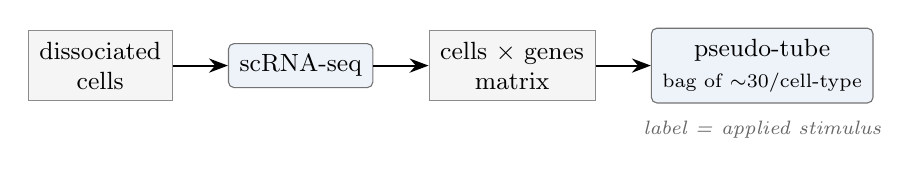
\begin{tikzpicture}[node distance=7mm]
  \node[data] (cells) {dissociated\\ cells};
  \node[box, right=of cells] (seq) {scRNA-seq};
  \node[data, right=of seq] (mat) {cells $\times$ genes\\ matrix};
  \node[box, right=of mat, fill=boxbg] (tube) {pseudo-tube\\ \scriptsize bag of $\sim$30/cell-type};
  \draw[ar] (cells)--(seq); \draw[ar] (seq)--(mat); \draw[ar] (mat)--(tube);
  \node[lbl, below=1mm of tube] {label = applied stimulus};
\end{tikzpicture}
\caption{Pre-processing. Cells are sequenced, normalised (total-count + log1p),
then assembled into stratified pseudo-tubes; the tube inherits the stimulus
label.}\label{fig:f4}
\end{figure}

\subsection{Two complementary datasets}
We use two datasets with opposite strengths (Table~\ref{tab:data}). Oesinghaus
(human PBMC, 91 cytokines, 24h) is broad but single-time. Sheu (mouse bone-marrow
macrophages, 7 stimuli, a true time-course) is narrow but has the \emph{time axis}
and textbook-clean cascade biology --- ideal for validating direction.

\begin{table}[h]\centering\small
\caption{The two datasets.}\label{tab:data}
\begin{tabular}{@{}lll@{}}
\toprule
 & \textbf{Oesinghaus 2024} & \textbf{Sheu 2024} \\
\midrule
organism / tissue   & human PBMC                 & mouse BMDM (macrophages) \\
stimuli             & 91 cytokines (+PBS)        & 7 (LPS, LPSlo, P3CSK, PIC, TNF, CpG, \ifnb) \\
time points         & 24h (single)               & 0/0.25/0.5/1/3/5/8/24h (course) \\
genes               & 4000 HVGs                  & 500-gene targeted panel \\
``donors''          & 12 biological donors       & 4 pseudo-donors @3h (context$\times$rep) \\
cells/tube          & $\sim$480 (16 cell types)  & $\sim$120 (mac\_c0--c3) \\
role here           & broad benchmark (Path B)   & single-frame, multi-time confirmation \\
\bottomrule
\end{tabular}
\end{table}

\subsection{The test cascades (textbook TLR biology)}
Sheu's stimuli are Toll-like-receptor (TLR) agonists with \emph{known} wiring
(Fig.~\ref{fig:f5}). Two adaptor arms matter: \textbf{TRIF} (engaged by TLR3 and
TLR4) $\to$ IRF3 $\to$ type-I interferon (\ifnb{}); and \textbf{MyD88} (TLR2/4/9)
$\to$ \nfkb{} $\to$ TNF. So \emph{polyIC} (TLR3) and \emph{LPS} (TLR4) drive
\ifnb{} (an IFN cascade), while \emph{LPS/LPSlo/P3CSK/CpG} drive autocrine TNF (an
\nfkb{} cascade). TLR2 (P3CSK) has \emph{no} TRIF arm, so P3CSK$\to$\ifnb{} is a
true negative. These give us crystal-clear directional labels
(Appendix~\ref{app:sheu}).

\begin{figure}[h]\centering
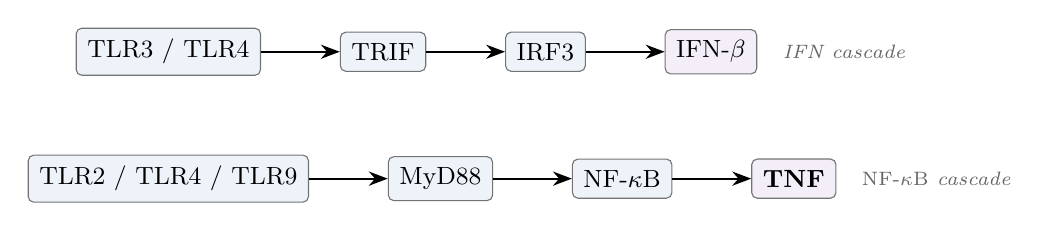
\begin{tikzpicture}[node distance=6mm and 10mm]
  \node[box] (t34) {TLR3 / TLR4};
  \node[box, right=of t34] (trif) {TRIF};
  \node[box, right=of trif] (irf3) {IRF3};
  \node[pbox, right=of irf3] (ifn) {\textbf{\ifnb}};
  \draw[ar] (t34)--(trif); \draw[ar] (trif)--(irf3); \draw[ar] (irf3)--(ifn);
  \node[box, below=10mm of t34] (t249) {TLR2 / TLR4 / TLR9};
  \node[box, right=of t249] (myd) {MyD88};
  \node[box, right=of myd] (nf) {\nfkb};
  \node[pbox, right=of nf] (tnf) {\textbf{TNF}};
  \draw[ar] (t249)--(myd); \draw[ar] (myd)--(nf); \draw[ar] (nf)--(tnf);
  \node[lbl, right=2mm of ifn] {IFN cascade};
  \node[lbl, right=2mm of tnf] {\nfkb{} cascade};
\end{tikzpicture}
\caption{The two adaptor arms. polyIC/LPS$\,\to\,$\ifnb{} (TRIF$\to$IRF3); the
MyD88 ligands $\to$ autocrine TNF. The two product signatures (ISGs vs.\ \nfkb{}
targets) are transcriptionally distinct --- the precondition our test needs.}
\label{fig:f5}
\end{figure}

% ================================================================== §4 method
\section{Method: the three-step pipeline}\label{sec:method}

\subsection{Overview}
The pipeline (Fig.~\ref{fig:f6}) chains three modules. \emph{Path A} uses a trained
AB-MIL model's latent geometry to propose coupled pairs. The \emph{Bridge} trains
one binary classifier per cytokine and uses Integrated Gradients to read out each
cytokine's gene signature \Sx{}. \emph{Path B} combines the signatures with the
cells to score direction. Path A and the Bridge both rest on the same AB-MIL
model, described next.

\begin{figure}[h]\centering
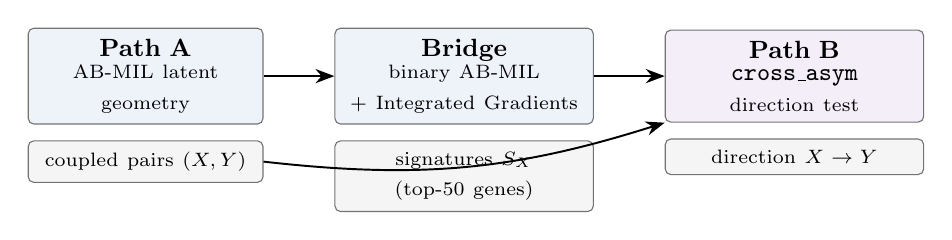
\begin{tikzpicture}[node distance=5mm and 9mm]
  \node[box, text width=2.7cm] (a) {\textbf{Path A}\\ \scriptsize AB-MIL latent\\ geometry};
  \node[box, below=2mm of a, text width=2.7cm, fill=black!4] (ao) {\scriptsize coupled pairs $(X,Y)$};
  \node[box, right=of a, text width=3.0cm] (b) {\textbf{Bridge}\\ \scriptsize binary AB-MIL\\ + Integrated Gradients};
  \node[box, below=2mm of b, text width=3.0cm, fill=black!4] (bo) {\scriptsize signatures $S_X$ (top-50 genes)};
  \node[pbox, right=of b, text width=3.0cm] (c) {\textbf{Path B}\\ \scriptsize \cross{}\\ direction test};
  \node[pbox, below=2mm of c, text width=3.0cm, fill=black!4] (co) {\scriptsize direction $X\!\to\!Y$};
  \draw[ar] (a)--(b); \draw[ar] (b)--(c);
  \draw[ar] (ao.east) to[bend right=12] (c.south west);
\end{tikzpicture}
\caption{The pipeline. Path A proposes \emph{which} pairs couple; the Bridge
discovers per-cytokine signatures; Path B assigns \emph{direction} to the coupled
pairs.}\label{fig:f6}
\end{figure}

\subsection{The AB-MIL model}\label{sec:mil}
A pseudo-tube is a bag $X\in\mathbb{R}^{N\times G}$ of $N$ cells over $G$ genes,
with one tube-level label. Attention-based multiple-instance learning
(Fig.~\ref{fig:f7}) maps each cell to an embedding, learns a soft attention weight
per cell, pools into one tube vector, and classifies:
\begin{align}
h_i &= \mathrm{InstanceEncoder}(x_i)\in\mathbb{R}^{d}, &
a_i &= \frac{\exp\!\big(w^{\top}\tanh(V h_i)\big)}{\sum_j \exp\!\big(w^{\top}\tanh(V h_j)\big)},\\
z &= \textstyle\sum_i a_i\, h_i, &
\hat y &= \mathrm{softmax}(W z + b).
\end{align}
The encoder is a residual MLP (LayerNorm\,$\to$\,Linear\,$\to$\,GELU blocks, skip
connections, \emph{no dropout} so attention is stable); the attention is the gated
form of Ilse et al.\ (2018). Training is two-stage: Stage 1 pre-trains the encoder
to classify cell types; Stage 2 freezes the encoder and trains attention\,+\,head
on the tube label. Exact dimensions and schedules are in Appendix~\ref{app:tech}.

\begin{figure}[h]\centering
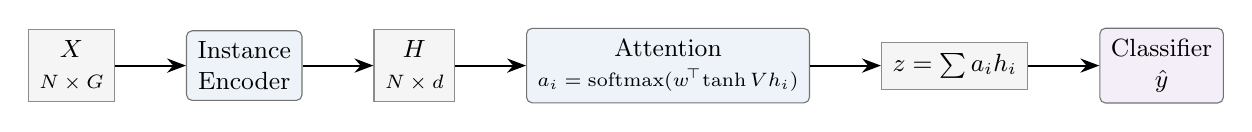
\begin{tikzpicture}[node distance=5mm and 9mm]
  \node[data] (x) {$X$\\ \scriptsize $N\times G$};
  \node[box, right=of x] (enc) {Instance\\Encoder};
  \node[data, right=of enc] (h) {$H$\\ \scriptsize $N\times d$};
  \node[box, right=of h] (att) {Attention\\ \scriptsize $a_i=\mathrm{softmax}(w^{\!\top}\!\tanh V h_i)$};
  \node[data, right=of att] (z) {$z=\sum a_i h_i$};
  \node[pbox, right=of z] (cl) {Classifier\\ $\hat y$};
  \draw[ar] (x)--(enc); \draw[ar] (enc)--(h); \draw[ar] (h)--(att);
  \draw[ar] (att)--(z); \draw[ar] (z)--(cl);
\end{tikzpicture}
\caption{AB-MIL forward pass. Cells $\to$ embeddings $\to$ attention pooling $\to$
tube vector $\to$ stimulus prediction.}\label{fig:f7}
\end{figure}

\subsection{Path A --- coupled pairs (brief)}
After Stage 2, we read the encoder's latent geometry: per cell type, how far each
cytokine's centroid is pushed toward another cytokine's, relative to the resting
(PBS) state. Pairs with significant mutual bias are ``coupled axes''. On
Oesinghaus this produced 121 axes ($\sim$50\% literature-supported). For this
report Path A is context; the spotlight is the Bridge and Path B.

\subsection{Bridge --- discovering signatures with Integrated Gradients}
For each cytokine $X$ we train a \emph{binary} AB-MIL classifier ($X$ vs.\ PBS).
\textbf{Integrated Gradients} (IG) then attributes the prediction to input genes:
it integrates the model's gradient along a straight line from a baseline tube
(the PBS per-gene mean) to the real tube (20-step midpoint rule), giving a
per-gene importance. Averaging over tubes and ranking yields \Sx{} $=$ the top-50
genes. Crucially \Sx{} is \emph{discovered from data}, not curated by hand.

\subsection{Path B --- direction, and the bug we fixed}\label{sec:pathb}
Given a coupled pair $(a,b)$ with signatures $S_a,S_b$, let $s(x,S)$ be the mean
expression of gene-set $S$ in $x$'s tubes (PBS-normalised). The original ``§24''
directional score was
\begin{equation}
\dscore = \underbrace{\big(s(a,S_a)-s(b,S_a)\big)}_{\text{asym on }S_a}
         -\underbrace{\big(s(a,S_b)-s(b,S_b)\big)}_{\text{asym on }S_b}
        = \big(s_aS_a+s_bS_b\big)-\big(s_aS_b+s_bS_a\big).
\end{equation}
Expanding shows it is \textbf{symmetric under swapping $a\leftrightarrow b$}: its
\emph{sign cannot encode direction} when the two ``pathways'' are the cytokines'
own signatures. This is exactly why our first runs scored at chance.

The direction lives in the \textbf{antisymmetric cross-engagement}:
\begin{equation}\label{eq:cross}
\boxed{\;\cross(a,b) \;=\; s(a,S_b)\;-\;s(b,S_a)\;}
\qquad\text{(PBS-normalised)}.
\end{equation}
It flips sign under $a\leftrightarrow b$. Its meaning is the cascade intuition
(Fig.~\ref{fig:f8}): if $a$ is upstream, $a$'s tubes carry $b$'s signature (via the
cascade) so $s(a,S_b)$ is high, while $b$'s tubes do \emph{not} carry $a$'s
signature so $s(b,S_a)$ is low $\Rightarrow$ \cross{}\,$>0\Rightarrow a$ upstream.
We aggregate the per-cell-type \cross{} by its median and report a sign-consensus
fraction; a permutation null with random gene-sets guards against the signatures
merely tracking activation level.

\begin{figure}[h]\centering
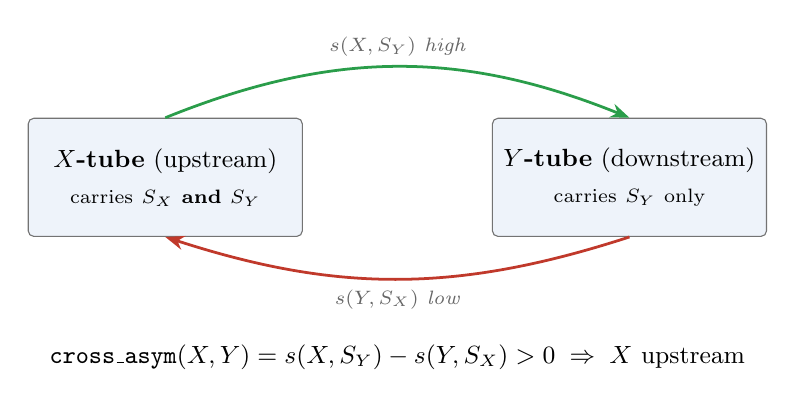
\begin{tikzpicture}[node distance=8mm]
  \node[box, text width=3.2cm, minimum height=1.5cm] (xt)
     {\textbf{$X$-tube} (upstream)\\[2pt] \scriptsize carries $S_X$ \textbf{and} $S_Y$};
  \node[box, text width=3.2cm, minimum height=1.5cm, right=24mm of xt] (yt)
     {\textbf{$Y$-tube} (downstream)\\[2pt] \scriptsize carries $S_Y$ only};
  \draw[ar, cgreen, line width=1pt] (xt.north) to[bend left=22]
        node[lbl, above]{$s(X,S_Y)$ high} (yt.north);
  \draw[ar, cred, line width=1pt] (yt.south) to[bend left=18]
        node[lbl, below, pos=0.5]{$s(Y,S_X)$ low} (xt.south);
  \node[below=20mm of $(xt)!0.5!(yt)$] {\small
     $\cross(X,Y)=s(X,S_Y)-s(Y,S_X)>0 \;\Rightarrow\; X$ upstream};
\end{tikzpicture}
\caption{Why \cross{} encodes direction. The upstream tube engages the downstream
signature more than vice versa; \dscore{} (symmetric) averages this away,
\cross{} (antisymmetric) keeps it.}\label{fig:f8}
\end{figure}

% ================================================================== §5 results
\section{Results}\label{sec:results}

\subsection{Oesinghaus 24h: 88\% vs.\ 47\%, same data}
We first hand-audited the human-PBMC literature labels (the automatic keyword tags
were noisy; 7 of 29 flipped under receptor-biology review), giving 17 cleanly
directional benchmark cascades. On \emph{identical} per-cell-type values, swapping
\dscore{} for \cross{} lifts directional sign-accuracy from \textbf{8/17 = 47\%}
(chance) to \textbf{15/17 = 88\%} (Fig.~\ref{fig:f9}, Table~\ref{tab:oes}). The
two misses both involve VEGF. A random-gene-set permutation null is cleared by 34
axes ($p<0.05$), and a label-permutation null on the benchmark gives $p=0.003$ ---
the discovered signatures carry genuine direction information, not just activation
magnitude. The per-axis breakdown (Fig.~\ref{fig:f10}) shows the sign is right
across diverse cascades (interferon, interleukin, growth-factor).

\begin{figure}[h]\centering
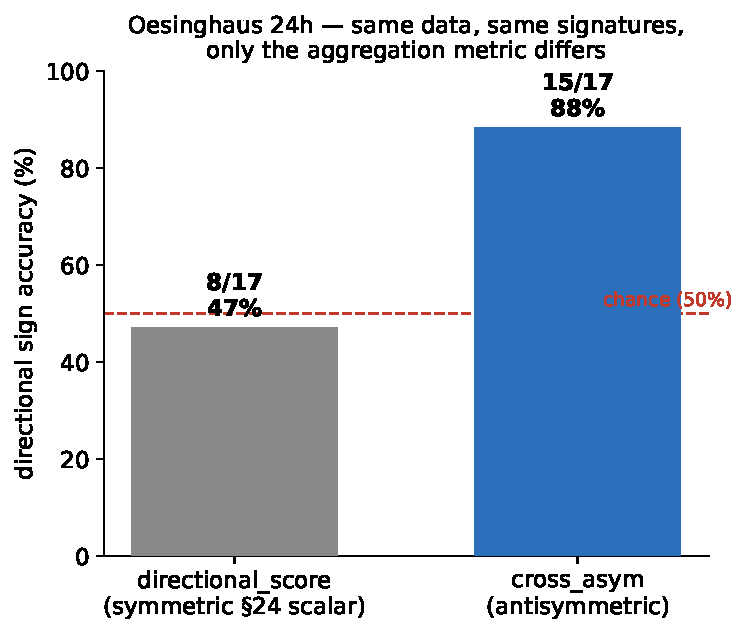
\includegraphics[width=0.52\linewidth]{figures/f9_oes_headline.pdf}
\hfill
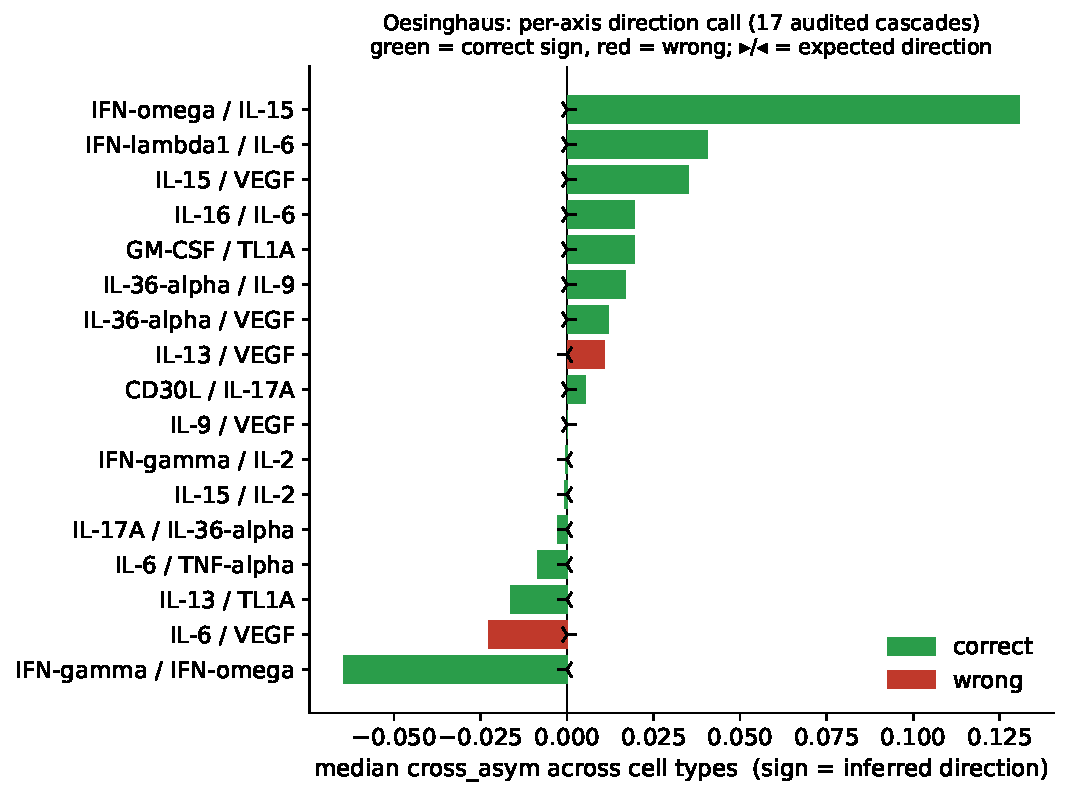
\includegraphics[width=0.45\linewidth]{figures/f10_oes_peraxis.pdf}
\caption{\textbf{Left (F9):} the headline --- the only change is the aggregation
metric. \textbf{Right (F10):} per-axis median \cross{} on the 17 audited cascades;
green = correct sign, red = wrong (both VEGF). $\blacktriangleright/\blacktriangleleft$
mark the expected direction.}\label{fig:f9}
\end{figure}
\addtocounter{figure}{0}\label{fig:f10}

\begin{table}[h]\centering\small
\caption{Oesinghaus 24h, 17 audited directional cascades.}\label{tab:oes}
\begin{tabular}{@{}lccc@{}}
\toprule
metric & a$\to$b (n=10) & b$\to$a (n=7) & total \\
\midrule
\dscore{} (symmetric) & --- & --- & 8/17 = 47\% \\
\cross{} (antisymmetric) & 9/10 = 90\% & 6/7 = 86\% & \textbf{15/17 = 88\%} \\
\bottomrule
\end{tabular}\\[2pt]
{\scriptsize 34/53 axes beat the random-gene-set null ($p<0.05$); benchmark
label-permutation $p=0.003$.}
\end{table}

\subsection{Sheu single-frame, multiple time points}
Each time point is analysed \emph{independently} --- no information from one frame
enters another (the core single-frame constraint). On crystal-clear TLR-biology
labels, directional accuracy is best at \textbf{5h: 6/7 = 86\%}
(Table~\ref{tab:sheu}, Fig.~\ref{fig:f12}). Two findings stand out
(Fig.~\ref{fig:f11}): (i) the \nfkb{}$\to$TNF cascades recover \emph{well} (4/4 at
5h) --- the opposite of the older curated-pathway approach, because the
data-discovered signatures separate TNF from the TLR ligands; (ii) one IFN cascade,
\textbf{polyIC$\to$\ifnb{}}, fails at \emph{every} time point.

\begin{figure}[h]\centering
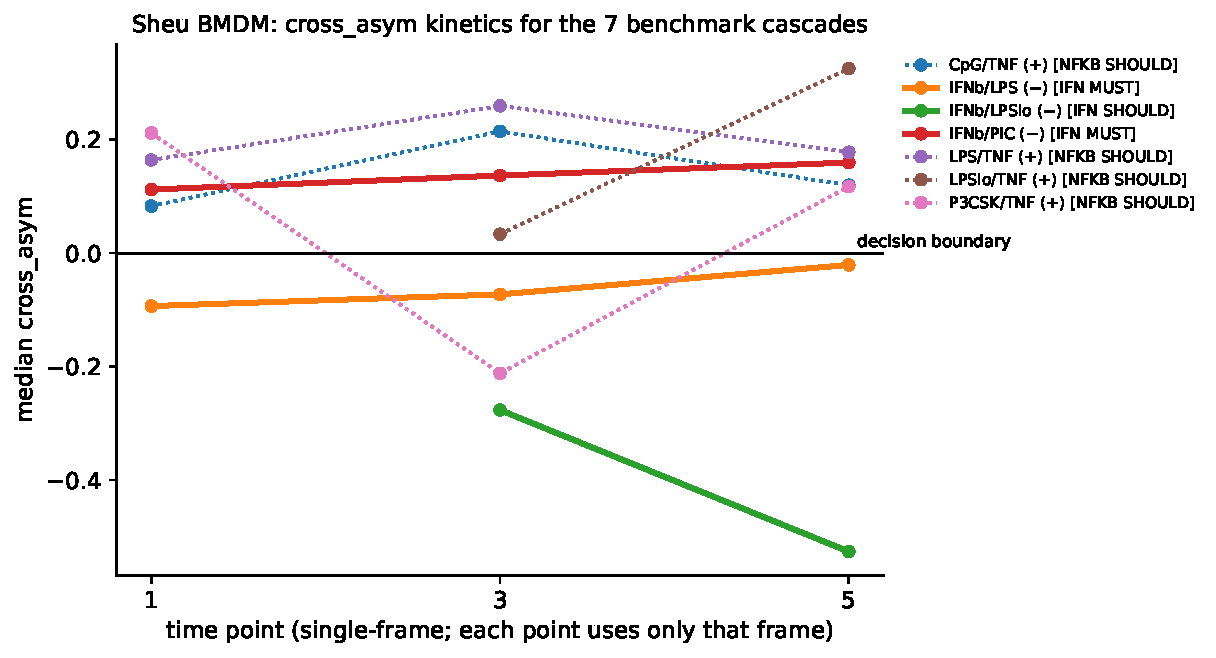
\includegraphics[width=0.62\linewidth]{figures/f11_sheu_kinetic.pdf}
\caption{(F11) \cross{} kinetics for the 7 Sheu benchmark cascades; $0$ is the
decision boundary. IFN cascades solid, \nfkb{} dotted. LPS/\ifnb{} sits correctly
below 0 at all times; polyIC/\ifnb{} sits wrongly above.}\label{fig:f11}
\end{figure}

\begin{table}[h]\centering\small
\caption{Sheu single-frame directional accuracy by class $\times$ time.}\label{tab:sheu}
\begin{tabular}{@{}lccc@{}}
\toprule
class & 1h & 3h & 5h \\
\midrule
IFN (MUST: LPS, polyIC $\to$\ifnb)   & 1/2 & 1/2 & 1/2 \\
IFN (SHOULD: LPSlo$\to$\ifnb)         & --- & 1/1 & 1/1 \\
\nfkb{} (SHOULD: $\cdot\to$TNF)       & 3/3 & 3/4 & 4/4 \\
\midrule
\textbf{all directional}              & 4/5 & 5/7 & \textbf{6/7} \\
\bottomrule
\end{tabular}
\end{table}

\begin{figure}[h]\centering
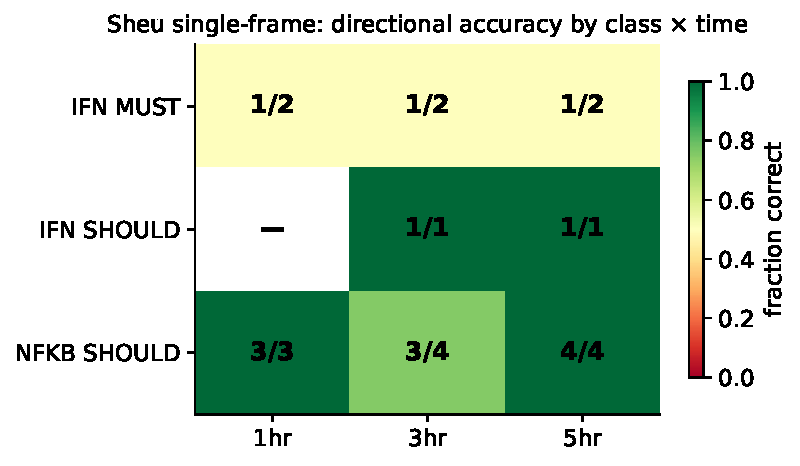
\includegraphics[width=0.46\linewidth]{figures/f12_sheu_heatmap.pdf}
\hfill
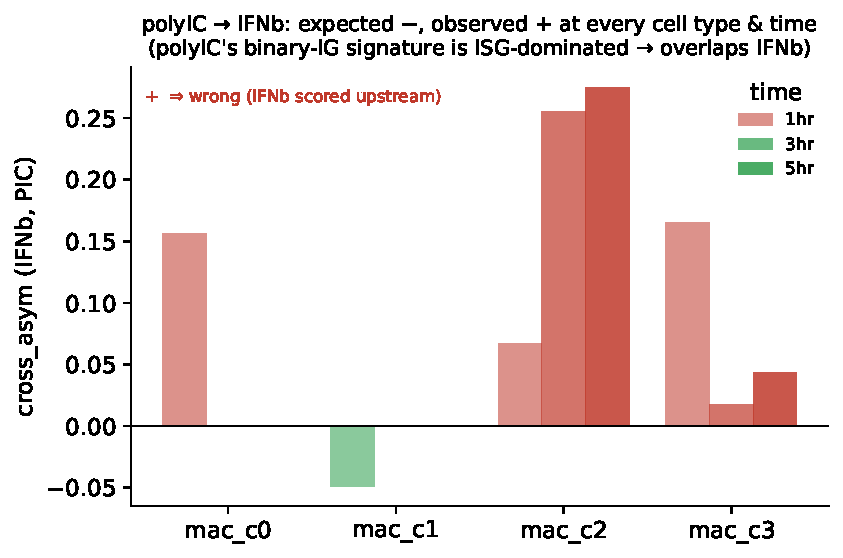
\includegraphics[width=0.49\linewidth]{figures/f13_polyic.pdf}
\caption{\textbf{Left (F12):} accuracy heatmap (class $\times$ time); 5h is best.
\textbf{Right (F13):} the polyIC$\to$\ifnb{} failure is consistent across all cell
types and times (all positive = wrong direction).}\label{fig:f12}
\end{figure}
\addtocounter{figure}{0}\label{fig:f13}

\subsection{Why polyIC$\to$\ifnb{} fails (and why that is informative)}
polyIC's \emph{discovered} signature is dominated by interferon-stimulated genes
(ISGs): those are the strongest differentially-expressed genes, far above the
lower-expressed IRF3-direct genes (\emph{Ifnb1}, \emph{Cxcl10}). So
$S_{\text{polyIC}}\approx S_{\ifnb}$, and \ifnb{} (which signals \emph{directly}
through its receptor) engages this shared ISG set more strongly than polyIC (which
reaches it only via the autocrine loop). The sign therefore inverts. LPS$\to$\ifnb{}
survives because LPS carries a broad non-ISG (\nfkb{}) program that keeps
$S_{\text{LPS}}$ distinct from $S_{\ifnb}$. This is a concrete, testable failure
mode (next steps, §\ref{sec:next}), not a mystery.

% ================================================================== §6 limits
\section{Honest limitations}\label{sec:limits}
\begin{itemize}[leftmargin=1.3em,itemsep=2pt]
\item \textbf{Direction, not existence.} \cross{} assigns a direction; it does
\emph{not} decide whether a cascade exists. No-cascade Sheu pairs also have large
$|\cross|$. That is by design: Path A decides \emph{which} pairs couple; \cross{}
only directs those.
\item \textbf{Small benchmarks.} 17 and 7 graded cascades. Sheu's IFN-MUST is
effectively one clean win (LPS) plus one explained failure (polyIC).
\item \textbf{Labels are a judgement call.} The 88\% is against \emph{our}
receptor-biology audit (7 tags flipped); the audit log is open for review.
\item \textbf{Retrospective.} We test on \emph{known} cascades; we have not yet
made a prospective, experimentally-validated prediction.
\end{itemize}

% ================================================================== §7 next
\section{Current state and next steps}\label{sec:next}
The method works at $\sim$86--88\% direction accuracy on two independent datasets,
including early time points, with a clean mechanistic story. Cheap next
experiments: (1) \textbf{polyIC ISG-exclusion test} --- re-derive
$S_{\text{polyIC}}$ with ISGs removed; we predict the sign flips to correct,
isolating the mechanism; (2) inspect the VEGF signature (the two Oesinghaus
misses); (3) run Path A$\to$Path B \emph{end-to-end} on Sheu (coupling then
direction); (4) sensitivity to the top-$n$ signature size. The big-picture goal is
a prospective prediction confirmed by a perturbation experiment.

% ================================================================== §8 talk
\section{Suggested 45-minute talk structure}\label{sec:talk}
\begin{table}[h]\centering\small
\caption{A 45+15 plan. Anchor on the four ``money'' figures (F2, F8, F9, F12).}
\begin{tabular}{@{}rll@{}}
\toprule
min & segment & key visual \\
\midrule
0--8   & biology primer + the question (why direction is hard/important) & F2, F3 \\
8--16  & data + test-cascade biology (TLR arms) & Table~1, F5 \\
16--31 & method: MIL $\to$ IG signatures $\to$ \cross{} (the symmetric-bug story) & F6, F7, \textbf{F8} \\
31--41 & results: Oesinghaus 88\%, Sheu kinetics, the polyIC wart & \textbf{F9}, F11, \textbf{F12} \\
41--45 & limitations + next steps & --- \\
45--60 & discussion & --- \\
\bottomrule
\end{tabular}
\end{table}

\appendix
% ================================================================== App A
\section{Full technical specifications}\label{app:tech}

\begin{table}[h]\centering\small
\caption{Model architecture (dimensions) across runs.}\label{tab:arch}
\begin{tabular}{@{}lccccc@{}}
\toprule
run & embed $d$ & enc.\ $h_0$ & enc.\ $h_1$ & att.\ hidden & classes \\
\midrule
Sheu Stage 1+2 (Path A)         & 32  & 512 & 256 & 16  & 8 \\
Sheu binary (Bridge)            & 128 & 256 & 128 & 64  & 2 \\
Oesinghaus binary (narrow, 8)   & 32  & 128 & 64  & 16  & 2 \\
Oesinghaus binary (wide, 16)    & 512 & 512 & 512 & 128 & 2 \\
\bottomrule
\end{tabular}\\[2pt]
{\scriptsize Encoder: input\_proj(LayerNorm,GELU) $\to$ ResBlock($h_0$) $\to$
DownBlock($h_0\!\to\!h_1$) $\to$ ResBlock($h_1$) $\to$ DownBlock($h_1\!\to\!d$);
GELU; Kaiming init; block fc2 zero-init (identity start); \textbf{no dropout}.
Attention: gated Ilse-2018, $V\!\in\!\mathbb{R}^{d\times\text{att}}$, $w$ linear,
Xavier init. Classifier: Linear$(d,K)$.}
\end{table}

\begin{table}[h]\centering\small
\caption{Training schedules (SGD, momentum 0.9).}\label{tab:sched}
\begin{tabular}{@{}lccccc@{}}
\toprule
run & S1 epochs & S1 lr & S2 epochs & S2 lr & warmup \\
\midrule
Sheu Stage 1+2 & 30 & 0.003 & 40  & 0.0005  & 5 \\
Sheu binary    & 20 & 0.005 & 200 & 0.0001  & --- \\
Oesinghaus binary (both) & 20 & 0.005 & 250 & 3e-5 & --- \\
\bottomrule
\end{tabular}\\[2pt]
{\scriptsize Stage 1 = encoder pre-train on cell types (batch 256); Stage 2 =
frozen-encoder MIL on tube labels (one tube per step). Sheu val pseudo-donor
M2\_IL4\_rep1; Oesinghaus val donors 2,3.}
\end{table}

\begin{table}[h]\centering\small
\caption{Bridge (IG), Path B, and pseudo-tube parameters.}\label{tab:params}
\begin{tabular}{@{}ll@{}}
\toprule
Integrated Gradients & baseline = PBS per-gene mean; 20-step midpoint rule;\\
 & $\le$10 tubes/cytokine; \Sx{} = top-50 by IG rank; CPU \\
Path B               & top\_n 50; min\_cells 10; n\_null\_perms 100; \\
 & magnitude\_threshold 0.01; strong/weak consensus 0.75/0.50 \\
pseudo-tubes         & 30 cells/cell-type; min 10 cells; 10 tubes/(stim,donor); \\
 & cell-typing by global Leiden on resting cells \\
\bottomrule
\end{tabular}
\end{table}

\paragraph{Key equations.} Encoder/attention/classifier as in §\ref{sec:mil}.
Integrated Gradients for gene $g$:
$\mathrm{IG}_g=(x_g-\bar x^{\,\text{PBS}}_g)\cdot\frac1n\sum_{k=1}^{n}
\partial_{x_g}f\big(\bar x^{\text{PBS}}+\alpha_k(x-\bar x^{\text{PBS}})\big)$,
$\alpha_k=\tfrac{k-0.5}{n}$. Direction:
$\cross(a,b)=\big(s(a,S_b)-s_{\text{PBS}}(S_b)\big)-\big(s(b,S_a)-s_{\text{PBS}}(S_a)\big)$,
sign $>0\Rightarrow a$ upstream.

% ================================================================== App B
\section{The 21 Sheu pairs (crystal-clear labels)}\label{app:sheu}
\begin{table}[h]\centering\small
\caption{Hand-curated from TLR receptor biology. Benchmark = the 7 directional
cascades scored; negatives test specificity; unknown = excluded.}
\begin{tabular}{@{}llp{8.6cm}@{}}
\toprule
pair & class & reason \\
\midrule
polyIC / \ifnb        & IFN MUST   & TLR3$\to$TRIF$\to$IRF3$\to$\ifnb{}; cleanest cascade \\
LPS / \ifnb           & IFN MUST   & LPS engages the TLR4--TRIF arm \\
LPSlo / \ifnb         & IFN SHOULD & low-dose LPS retains TRIF arm (weaker) \\
LPS / TNF             & \nfkb{} SHOULD & TLR4$\to$\nfkb{}$\to$autocrine TNF \\
LPSlo / TNF           & \nfkb{} SHOULD & low-dose TLR4$\to$\nfkb{}$\to$TNF \\
P3CSK / TNF           & \nfkb{} SHOULD & TLR2$\to$\nfkb{}$\to$TNF \\
CpG / TNF             & \nfkb{} SHOULD & TLR9$\to$\nfkb{}$\to$TNF \\
\midrule
P3CSK / \ifnb         & NEGATIVE   & TLR2 has no TRIF arm $\Rightarrow$ no \ifnb{} \\
CpG / \ifnb           & NEGATIVE   & TLR9 type-I IFN is pDC-restricted; minimal in BMDM \\
TNF / \ifnb           & NEGATIVE   & no TNF$\to$\ifnb{} cross-induction in macrophages \\
LPS / LPSlo           & NEGATIVE   & same receptor, dose difference --- not a cascade \\
\midrule
\multicolumn{3}{@{}p{12.6cm}@{}}{\emph{Plus 10 cross-receptor / MyD88-overlap pairs} (CpG/LPS, LPS/polyIC, \dots) $=$ \textbf{UNKNOWN} (excluded from scoring).}\\
\bottomrule
\end{tabular}
\end{table}

\vfill
{\footnotesize Reproducibility: figures from \code{scripts/make\_report\_figures.py};
results from \code{run\_pipeline\_a\_bridge\_b(\_sheu).py} +
\code{retally\_pipeline\_against\_audit.py}; labels in
\code{reports/sheu\_cascade/} and \code{reports/cascade\_pairs/}. Full session
narrative: \code{reports/SESSION\_SUMMARY\_2026-05-31.md}.}

\end{document}
